\documentclass{beamer}
\usepackage{beamerthemesplit} % new

\usepackage[utf8]{inputenc}

\begin{document}
\title{Perdidos en la ignorancia}
\author{ES\_2019\_G43-2-02}
\date{\today}

\frame{\titlepage}

\frame{\frametitle{Table of contents}\tableofcontents}


\section{Membres del equip}
\frame{\frametitle{Team}
  \begin{itemize}
    \item Adrián Moreno Gimeno
    \item Daniel Montesinos Santos
    \item Núria Navarro Juliana
    \item Aleksandra Jovanovic
    \item Desirée Pasión Rodriguez Sanchez
  \end{itemize}
}

\section{Joc}
\frame{\frametitle{Descripció}
Se trata de un juego basado en habitaciones, donde la única forma de pasar los niveles será solucionando los puzzles propuestos. Los mejores jugadores formarán parte del ranking, ordenados por tiempo y nivel alcanzado.
}

\section{Jira}
\subsection{Product Backlog/Tasques}
\frame{\frametitle{Product Backlog}
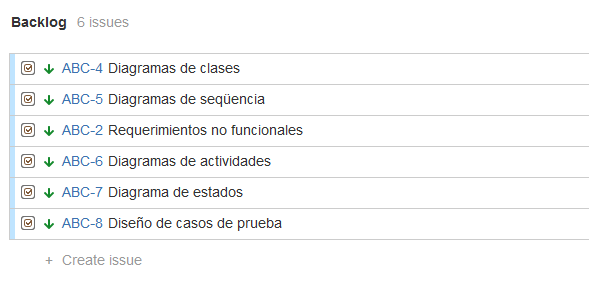
\includegraphics[width=1\textwidth]{./imatges/ProductBacklog.png}
}

\frame{\frametitle{Tasques}
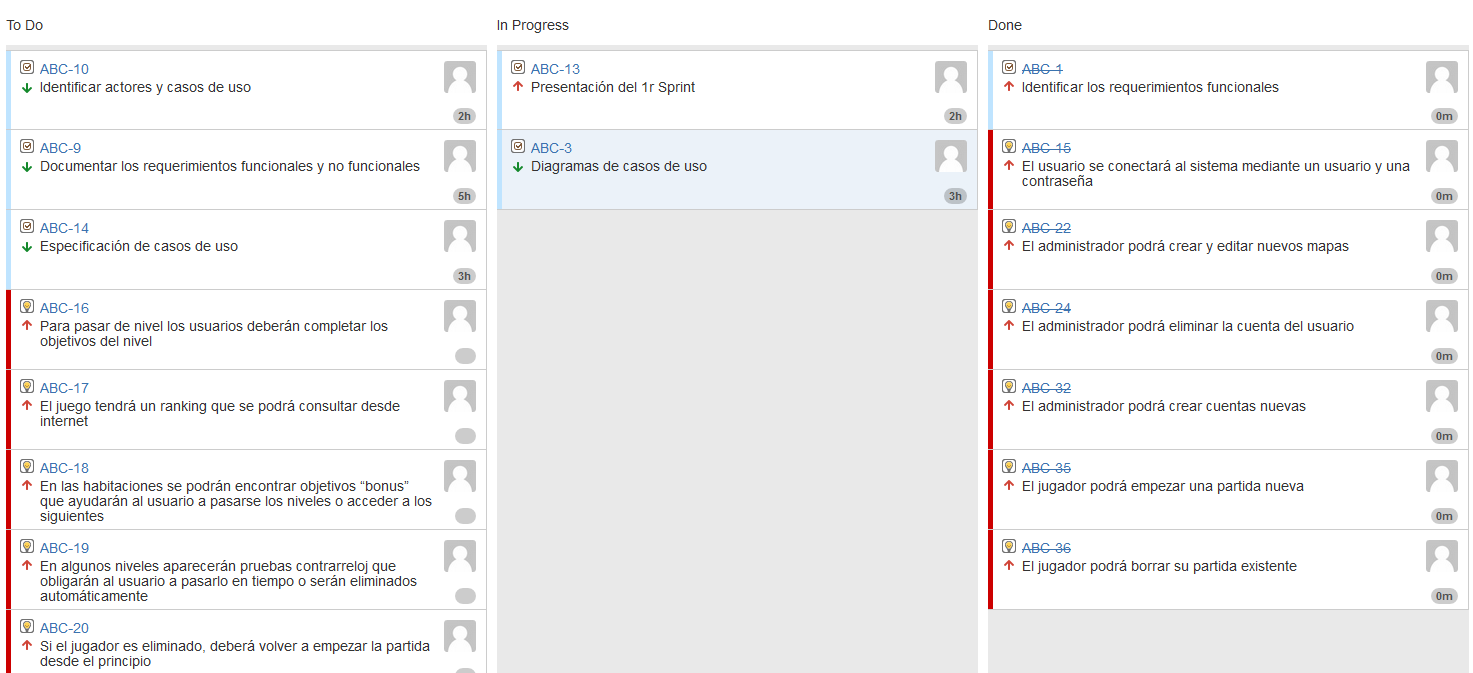
\includegraphics[width=1\textwidth]{./imatges/ProductBacklogSprint1.png}
}

\subsection{Burndown chart}
\frame{\frametitle{Burndown chart}
FALTA ACABARLO

  \begin{figure}[ht]
  \centering
  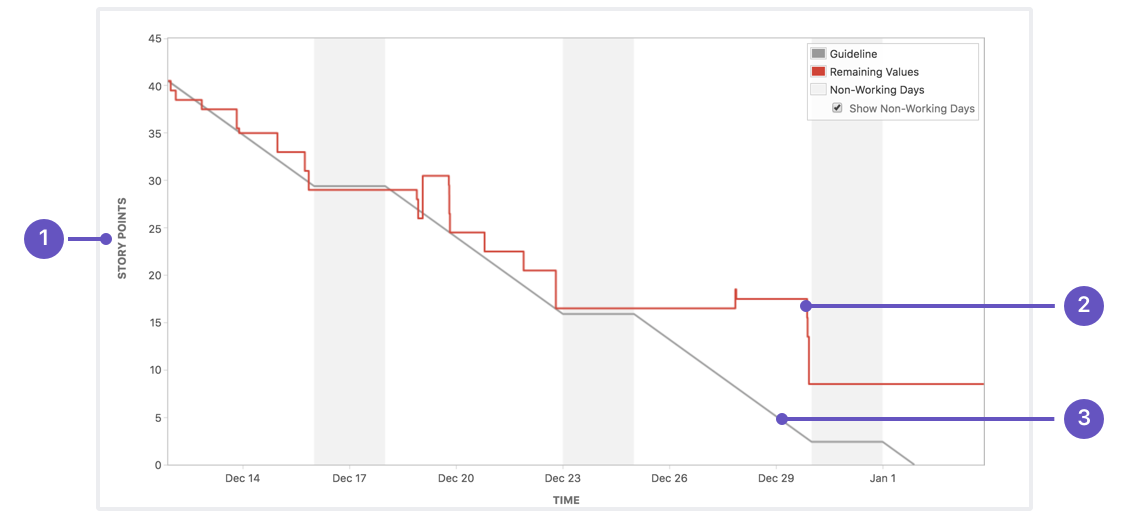
\includegraphics[width=1.1\textwidth]{./imatges/burndown-tutorial_02.png}
  \label{fig:bdchart}
\end{figure}

}

\section{Bitbucket}
\frame{\frametitle{Bitbucket}
}

\section{Especificacions}
\subsection{Requeriments}
\frame{\frametitle{Requeriments}
}

\subsection{Casos d'ús}
\frame{\frametitle{Diagrama}

  \begin{figure}[ht]
  \centering
  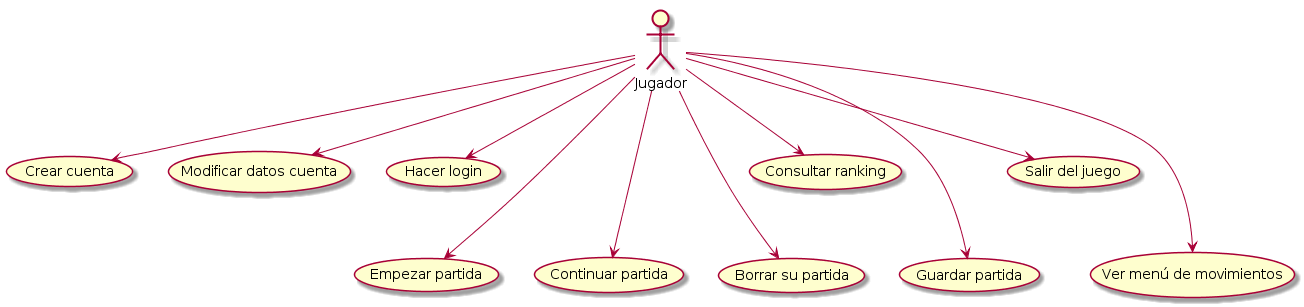
\includegraphics[width=1\textwidth]{./imatges/Jugador.png}
  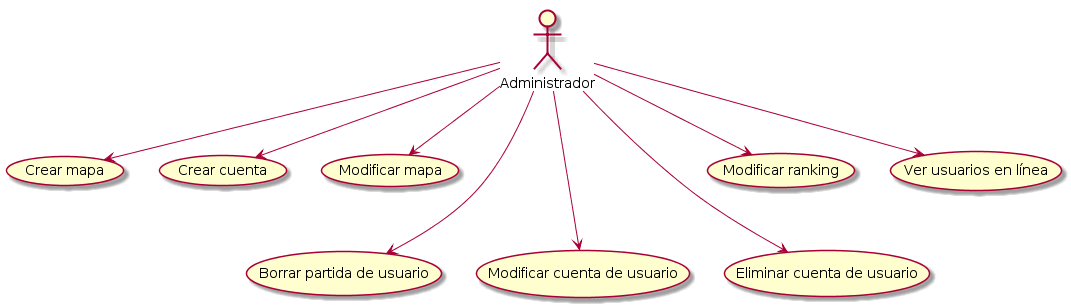
\includegraphics[width=1\textwidth]{./imatges/Administrador.png}
  \label{fig:usecase}
   \end{figure}
}

\frame{\frametitle{Casos d'ús (especificacions)}
\begin{center}
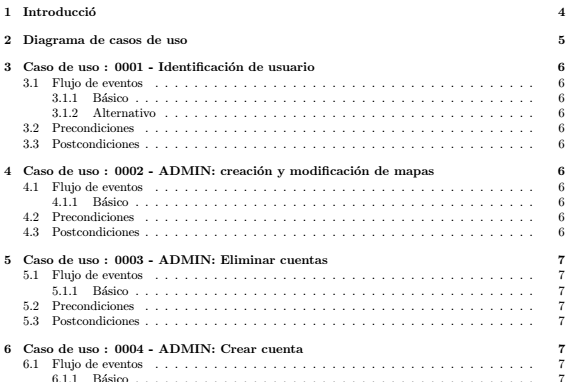
\includegraphics[width=0.7\textwidth]{./imatges/Especificaciones.png}

\end{center}}

\section{Conclusions}
\frame{\frametitle{Conclusions}
}

\end{document}
